\documentclass[10.5pt,a4paper]{article}
\usepackage[margin=1.8cm]{geometry}
\usepackage{fontspec}
\setmainfont{DejaVu Sans}
\setmonofont{DejaVu Sans Mono}[Scale=0.9]
\usepackage{unicode-math}
\setmathfont{DejaVu Math TeX Gyre}
\usepackage{graphicx,enumitem,xcolor,booktabs}
\pagestyle{empty}
\setlength{\parindent}{0pt}
\setlist[enumerate]{label=\alph*),leftmargin=1.4em,itemsep=0pt}
\newcommand{\resp}[1]{\par\vspace{#1}}
\newcommand{\preg}[1]{\vspace{4pt}{\large\bfseries #1}\par\vspace{3pt}}
\begin{document}
{\Large\bfseries SI7011 · Evento evaluativo 2 · Parte A: leer la evidencia}\par\vspace{10pt}
\textbf{Nombre:} \rule{8cm}{0.4pt}\hfill\textbf{Documento:} \rule{4cm}{0.4pt}\par\vspace{8pt}
\textbf{Individual · sin computador ni apuntes · 30 minutos · 6 preguntas, 1 punto cada una.}
Respuestas cortas: una o dos frases por literal. Cuando la pregunta pide evidencia, cita un número leído de la figura o la tabla.
Todos los resultados son de corridas reales de los notebooks de la sesión 03.
\vspace{6pt}\hrule\vspace{6pt}

\preg{1. Permutar los píxeles}
Uno de los modelos es un MLP sobre la imagen aplanada y el otro una CNN pequeña. «Permutados» quiere decir que se baraja el orden de los píxeles con \textbf{una misma permutación fija} para todas las imágenes (entrenamiento y validación) y se entrena de nuevo.\par
\begin{center}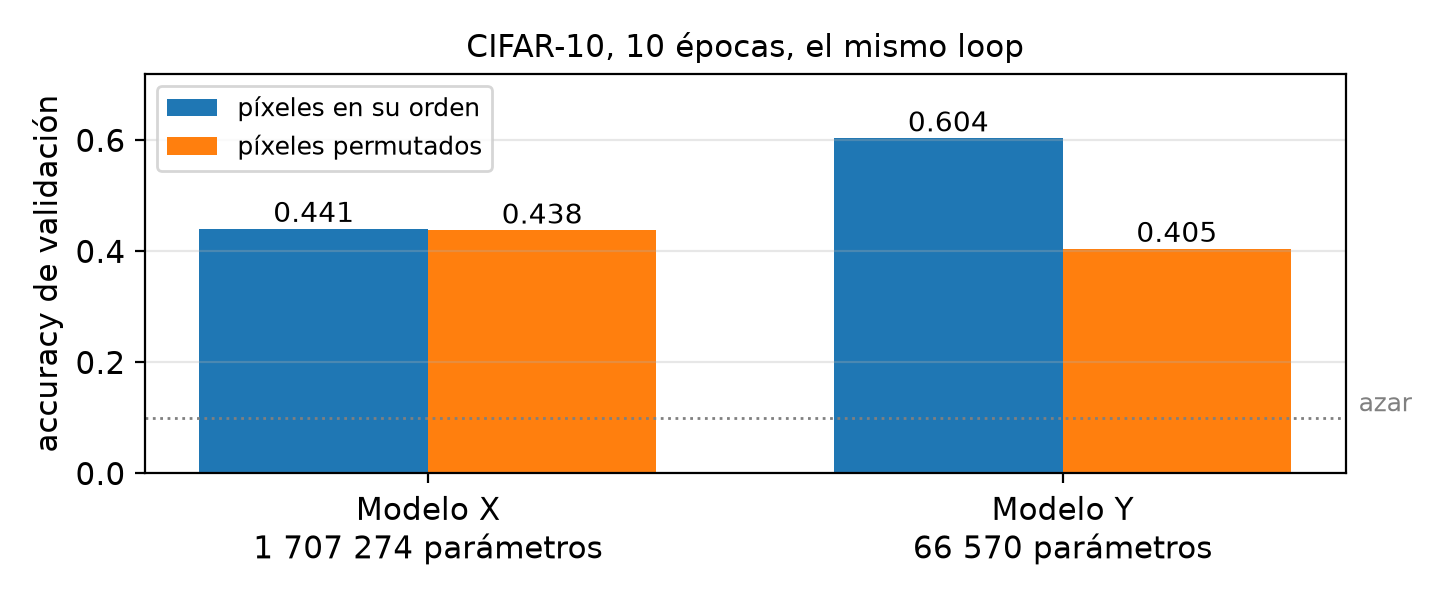
\includegraphics[width=0.66\linewidth]{fig1_permutacion.png}\end{center}
\begin{enumerate}
\item ¿Cuál es el MLP y cuál la CNN? Justifica con dos números de la figura.\resp{2.0cm}
\item ¿Por qué la permutación casi no afecta a uno y sí al otro? Nombra la suposición sobre la imagen que se rompe.\resp{2.2cm}
\end{enumerate}

\preg{2. Formas, parámetros y campo receptivo}
Una imagen de EuroSAT de $3\times64\times64$ entra a:\par\vspace{2pt}
\hspace*{1em}\texttt{Conv2d(3, 32, kernel\_size=3, padding=1)} → ReLU →\\
\hspace*{1em}\texttt{Conv2d(32, 64, kernel\_size=3, padding=1, stride=2)} → ReLU → \texttt{MaxPool2d(2)}
\begin{enumerate}
\item Escribe la forma $C\times H\times W$ de la salida de cada una de las tres capas.\resp{1.4cm}
\item ¿Cuántos parámetros tiene la segunda convolución? ¿Cuántos tendría una capa densa con la misma entrada y la misma salida? ¿Qué dos propiedades de la convolución explican la diferencia?\resp{2.2cm}
\item ¿Qué región de la imagen de entrada ve una posición a la salida de la segunda convolución? ¿Y a la salida del \texttt{MaxPool2d}?\resp{1.2cm}
\end{enumerate}

\newpage
\preg{3. BatchNorm y data augmentation}
Las tres corridas usan la misma red de bloques VGG: una \textbf{sin} BatchNorm, otra \textbf{con} BatchNorm, y otra con BatchNorm \textbf{y} data augmentation (recortes y flip horizontal).\par
\begin{center}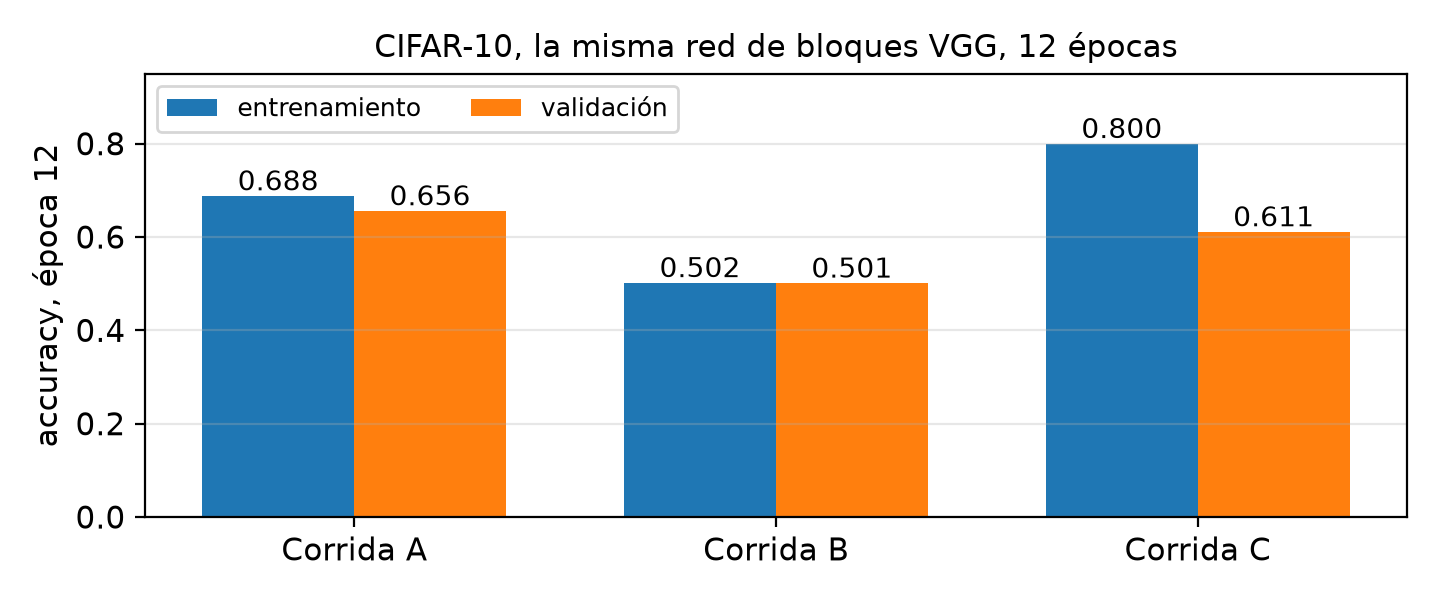
\includegraphics[width=0.66\linewidth]{fig2_bn_aug.png}\end{center}
\begin{enumerate}
\item Asigna A, B y C. Justifica cada una con un número de la figura.\resp{2.4cm}
\item Una corrida tiene \textbf{menos} accuracy de entrenamiento que otra pero \textbf{más} en validación. Explica por qué, y di qué número calcularías para mostrarlo.\resp{2.4cm}
\end{enumerate}

\preg{4. Profundidad y atajos}
Dos redes de 20 capas convolucionales con BatchNorm, sobre CIFAR-10: las mismas convoluciones, la misma inicialización, los mismos datos y la misma augmentation, 8 épocas. Una tiene atajos residuales y la otra no.\par\vspace{4pt}
\begin{center}
\begin{tabular}{lrrrr}
\toprule
 & parámetros & pérdida de entrenamiento & acc. entrenamiento & acc. validación \\
\midrule
Red P & 269\,722 & 1.189 & 0.565 & 0.529 \\
Red Q & 272\,474 & 0.992 & 0.639 & 0.606 \\
\bottomrule
\end{tabular}
\end{center}
\begin{enumerate}
\item Un compañero dice: «la red P sobreajusta». ¿Estás de acuerdo? Justifica con dos números de la tabla.\resp{2.0cm}
\item ¿Cuál red tiene atajos? Escribe la salida de un bloque residual en función de su entrada $a_l$ y explica por qué el atajo ayuda a entrenar una red profunda.\resp{2.4cm}
\item Q tiene 2\,752 parámetros más que P. ¿De dónde salen, si los atajos suelen ser la identidad?\resp{1.2cm}
\end{enumerate}

\newpage
\preg{5. Tres estrategias de transfer learning}
Una ResNet-18 sobre Oxford-IIIT Pets (37 razas) con tres estrategias: entrenar \textbf{desde cero}, \emph{linear probe} sobre el backbone de ImageNet \textbf{congelado}, y \emph{fine-tuning} de toda la red partiendo de ImageNet.\par
\begin{center}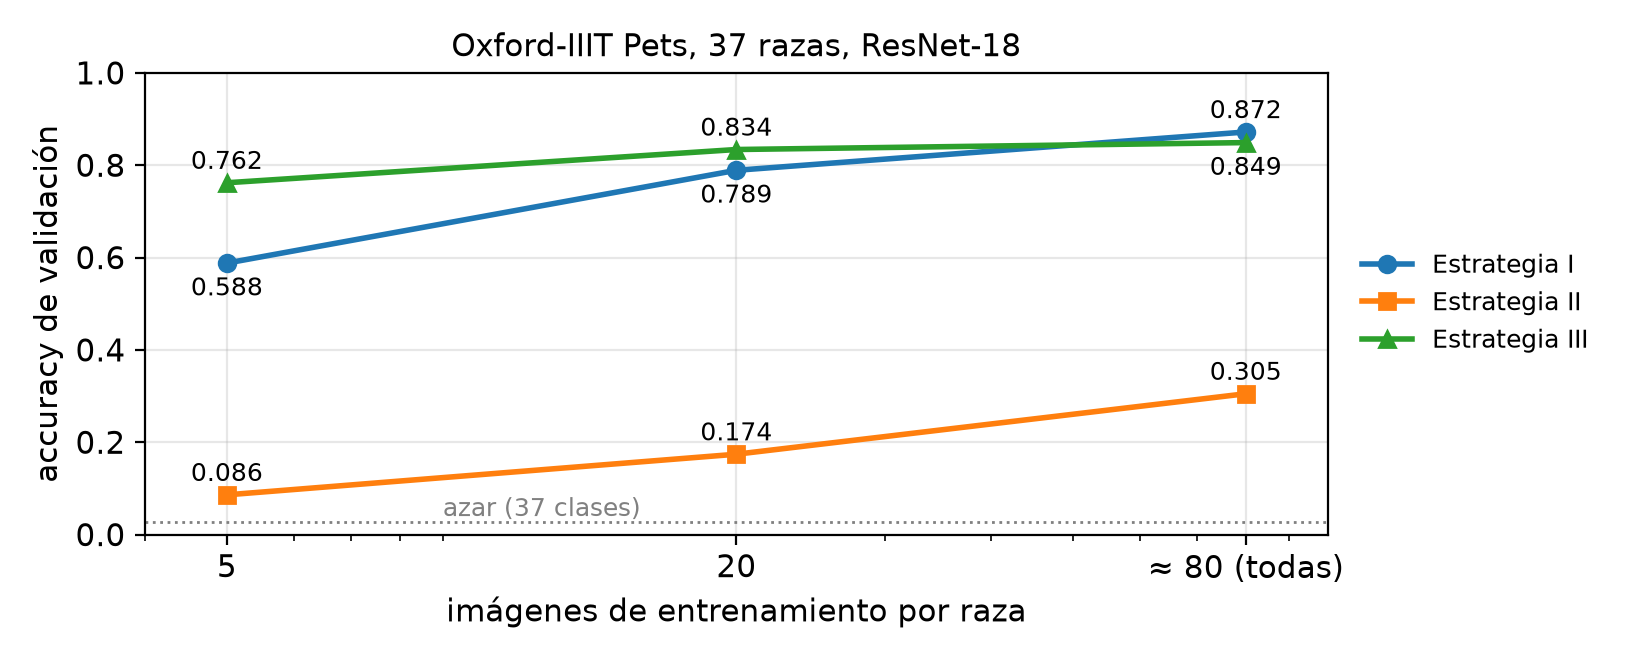
\includegraphics[width=0.72\linewidth]{fig3_transfer.png}\end{center}
\begin{enumerate}
\item Asigna I, II y III. Justifica cada una con un número de la figura.\resp{4.0cm}
\item Con 5 imágenes por raza, I queda por debajo de III; con todas, la supera. Explica por qué.\resp{4.5cm}
\item En el fine-tuning, el backbone usa $\eta=10^{-4}$ y la cabeza nueva $\eta=10^{-3}$. ¿Por qué no usar el mismo $\eta$ para toda la red?\resp{3.5cm}
\end{enumerate}

\newpage
\preg{6. CNN frente a ViT}
CIFAR-10, 50\,000 imágenes de entrenamiento. Las tres primeras filas se entrenan desde cero con el mismo loop durante 20 épocas.\par\vspace{4pt}
\begin{center}
\begin{tabular}{lrrr}
\toprule
Modelo & parámetros & acc. validación & tiempo \\
\midrule
CNN (bloques VGG + BatchNorm) & 72\,954 & 0.693 & 21 s \\
ViT pequeño (patches $4\times4$, $d=128$, 6 bloques) & 811\,146 & 0.603 & 75 s \\
El mismo ViT sin embeddings de posición & 811\,146 & 0.551 & 78 s \\
ViT-B/16 preentrenado en ImageNet + \emph{linear probe} & $\approx 86$ M & 0.943 & — \\
\bottomrule
\end{tabular}
\end{center}
\begin{enumerate}
\item El ViT pequeño tiene 11 veces más parámetros y aun así pierde contra la CNN, pero el ViT-B/16 preentrenado le gana. Explica las dos cosas.\resp{5.0cm}
\item Sin embeddings de posición, ¿qué información pierde el modelo? ¿Por qué aun así queda muy por encima del azar (0.10)?\resp{4.5cm}
\item Con imágenes de $32\times32$ y patches de $4\times4$, ¿cuántos tokens entran al Transformer, contando \texttt{[CLS]}? Con imágenes de $64\times64$ y los mismos patches, ¿cuántos, y por qué factor crece la matriz de atención?\resp{2.0cm}
\end{enumerate}

\end{document}
